\documentclass[10pt,letterpaper]{amspset}
\usepackage{fullpage}
\usepackage{gensymb}
\usepackage{graphicx}
\usepackage{tikz}
\usepackage{amsmath}
\usepackage{pgfplots}
\usepackage{amsthm}
\usepackage{amssymb}
\pgfplotsset{compat=1.17}
\graphicspath{ {./images/} }
\notag

% info for header block in upper right hand corner
\name{Brady Lamson}
\class{MATH 1120 SPRING 2021}
\assignment{Solving Complicated Trigonometric Equations and Inequalities Part II}
\duedate{Mar 7th}
\begin{document}

\problemlist{Solving Complicated Trigonometric Equations and Inequalities Part II: 

Section 10.7: 1--10, 20--30, 40--50, 57--65, 70--80}

\hrule \medskip
In exercises 1--10, find all of the exact solutions of the equation and then list those solutions which are in the interval $[0, 2\pi)$. \medskip
\hrule

\begin{problem}[1]
    $sin(5x) = 0$
\end{problem}

\begin{solution}
    First we'll go ahead and let $5x = \theta$ and we know the following information about sine:
    
    $sin(\theta) = 0$ when $\theta = 0, \pi, 2\pi, 3\pi, etc...$
    
    \begin{align}
        5x &= 0, \; x = 0 \\
        5x &= \pi, \; x = \frac{\pi}{5} \\
        5x &= 2\pi, \; x = \frac{2\pi}{5} \\
        5x &= 3\pi, \; x = \frac{3\pi}{5}
    \end{align}
    
    From this we can state that when $x = \frac{k \pi}{5} \rightarrow sin(5x) = 0$. So, for $[0, 2\pi)$ 
    
    \[\boxed{ x = \frac{k\pi}{5} \; for \; 0 \leq k \leq 9 }\]
    
    Why 9? Well, think about it. $\frac{10\pi}{5} = 2\pi$ which is not included in our range.
\end{solution}


\pagebreak


\begin{problem}[2]
    $cos(3x) = \frac{1}{2}$
\end{problem}

\begin{solution}
    \[Let \; 3x = \theta\]
    
    \[cos(\theta) = \frac{1}{2} \; when \; \theta = \frac{\pi}{3}, \frac{5\pi}{3}, \frac{7\pi}{3}, \frac{11\pi}{3}, \frac{13\pi}{3}, \frac{17\pi}{3}, ...\]
    
    \begin{align}
        3x &= \frac{\pi}{3}, \; x = \frac{\pi}{9} && 3x = \frac{5\pi}{3}, \; x = \frac{5\pi}{9} \\[+3mm]
        3x &= \frac{7\pi}{3}, \; x = \frac{7\pi}{9} && 3x = \frac{11\pi}{3}, \; x = \frac{11\pi}{9}\\[+3mm]
        3x &= \frac{13\pi}{3}, \; x = \frac{13\pi}{9} && 3x = \frac{17\pi}{3}, \; x = \frac{17\pi}{9} \\
    \end{align}
    
    \[\boxed{  x = \frac{\pi}{9}, \frac{5\pi}{9}, \frac{7\pi}{9}, \frac{11\pi}{9}, \frac{13\pi}{9}, \frac{17\pi}{9} \; when \; 0 \leq x \leq 2\pi  }\]
\end{solution}


\begin{problem}[3]
    $sin(-2x) = \frac{\sqrt{3}}{2}$
\end{problem}

\begin{solution}
    \[Let -2x = \theta\] 
    
    Keep in mind, now that we've got a negative $\theta$ we'll be going clockwise through the unit circle. 
    
    \[sin(\theta) = \frac{\sqrt{3}}{2} \; when \; \theta = -\frac{4\pi}{3}, -\frac{5\pi}{3}, -\frac{10\pi}{3}, -\frac{11\pi}{3} \]
    
    \begin{align}
        -2x &= -\frac{4\pi}{3}, \; x = \frac{2\pi}{3} && -2x = -\frac{5\pi}{3}, \; x = \frac{5\pi}{6}\\[+3mm]
        =2x &= -\frac{10\pi}{3}, \; x = \frac{5\pi}{3} && -2x = -\frac{11\pi}{3}, \; x = \frac{11\pi}{6}\\
    \end{align}
    
\[\boxed{ x = \frac{2\pi}{3} + \pi k \; or \; x = \frac{5\pi}{6} + \pi k \; when \; 0 \leq x \leq 2\pi }\]
\[\boxed{ x = \frac{2\pi}{3}, \frac{5\pi}{6}, \frac{5\pi}{3}, \frac{11\pi}{6} \; when \; 0 \leq x \leq 2\pi  }\]
\end{solution}


\pagebreak


\begin{problem}[4]
    $tan(6x) = 1$
\end{problem}

\begin{solution}
    \[Let \; 6x = \theta\] 

    So two things we need to consider: When is $tan(\theta)$ positive and when is $tan(\theta) = 1$? The answer to the first is quadrants 1 and 3. The answer to the second is when both sine and cosine are the same. 

    \[tan(\theta) = 1 \; when \; \theta = \frac{\pi}{4}, \frac{5\pi}{4}, \frac{9\pi}{4}, \frac{13\pi}{4}, ... \]
    
    \begin{align}
        6x &= \frac{\pi}{4}, \; x = \frac{\pi}{24} && 6x = \frac{5\pi}{4}, \; x = \frac{5\pi}{24}\\[+3mm]
        6x &= \frac{9\pi}{4}, \; x = \frac{3\pi}{8} && 6x = \frac{13\pi}{4}, \; x = \frac{13\pi}{24}\\[+3mm]
        6x &= \frac{17\pi}{4}, \; x = \frac{17\pi}{24} && 6x = \frac{21\pi}{4}, \; x = \frac{7\pi}{8}\\[+3mm]
        6x &= \frac{25\pi}{4}, \; x = \frac{25\pi}{24} && 6x = \frac{29\pi}{4}, \; x = \frac{29\pi}{24}\\[+3mm]
        6x &= \frac{33\pi}{4}, \; x = \frac{11\pi}{8} && 6x = \frac{37\pi}{4}, \; x = \frac{37\pi}{24}\\[+3mm]
        6x &= \frac{41\pi}{4}, \; x = \frac{41\pi}{24} && 6x = \frac{45\pi}{4}, \; x = \frac{15\pi}{8}\\
    \end{align}
    
\[\boxed{ x = \frac{\pi}{24} + \frac{\pi k}{6}  \; when \; 0 \leq x \leq 2\pi }\]
\[\boxed{ x = \frac{\pi}{24}, \frac{5\pi}{24}, \frac{3\pi}{8}, \frac{13\pi}{24}, \frac{17\pi}{24}, \frac{7\pi}{8}, \frac{25\pi}{24}, \frac{29\pi}{24}, \frac{11\pi}{8}, \frac{37\pi}{24}, \frac{41\pi}{24}, \frac{15\pi}{8} \; when \; 0 \leq x \leq 2\pi   }  \]
\end{solution}


\pagebreak


\begin{problem}[5]
    $csc(4x) = -1$
\end{problem}

\begin{solution}
   \[Let \; \theta = 4x\]
   
    \[csc(\theta) = \frac{1}{sin(\theta)}\]
    
    \[\frac{1}{sin(\theta)} = -1 \; when \; \theta = \frac{3\pi}{2}, \frac{7\pi}{2}, \frac{11\pi}{2}, \frac{15\pi}{2},\]
    
    \begin{align}
        4x &= \frac{3\pi}{2}, \; x = \frac{3\pi}{8} && 4x = \frac{7\pi}{2}, \; x = \frac{7\pi}{8}\\[+3mm]
        4x &= \frac{11\pi}{2}, \; x = \frac{11\pi}{8} && 4x = \frac{15\pi}{2}, \; x = \frac{15\pi}{8}\\
    \end{align}
    
\[\boxed{ x = \frac{3\pi}{8} + \frac{\pi k}{2}}\]
\[\boxed{ x = \frac{3\pi}{8}, \frac{7\pi}{8}, \frac{11\pi}{8}, \frac{15\pi}{8} \; when \; 0 \leq x \leq 2\pi  }\]
\end{solution}


\begin{problem}[6]
    $sec(3x) = \sqrt{2}$
\end{problem}

\begin{solution}
   \[let \; \theta = 3x\]
   
   \[\frac{1}{cos(\theta)} = \sqrt{2} \; when \; \theta = \frac{\pi}{4}, \frac{7\pi}{4}, \frac{9\pi}{4}, \frac{15\pi}{4}, \frac{17\pi}{4}, \frac{23\pi}{4}\]
       
    \begin{align}
        3x &= \frac{\pi}{4}, \; x = \frac{\pi}{12} && 3x = \frac{7\pi}{4}, \; x = \frac{7\pi}{12}\\[+3mm]
        3x &= \frac{9\pi}{4}, \; x = \frac{3\pi}{4} && 3x = \frac{15\pi}{4}, \; x = \frac{5\pi}{4}\\[+3mm]
        3x &= \frac{17\pi}{4}, \; x = \frac{17\pi}{12} && 3x = \frac{23\pi}{4}, \; x = \frac{23\pi}{12}\\
    \end{align}
    
    \[\boxed{ x = \frac{\pi}{12} + \frac{2\pi k}{3} \; or \; x = \frac{7\pi}{12} + \frac{2\pi k}{3}}\]
    \[\boxed{ x = \frac{\pi}{12}, \frac{7\pi}{12}, \frac{3\pi}{4}, \frac{5\pi}{4}, \frac{17\pi}{12}, \frac{23\pi}{12} \; when \; 0 \leq x \leq 2\pi  }\]
\end{solution}


\pagebreak


\begin{problem}[7]
    $cot(2x) = -\frac{\sqrt{3}}{3}$
\end{problem}

\begin{solution}
   \[\text{Let} \; \theta = 2x\]
   
   \[cot(\theta) = \frac{cos(\theta)}{sin(\theta)} = -\frac{\sqrt{3}}{3} \; \text{when} \; cos(\theta) = \pm \frac{1}{2} \; \text{and} \; sin(\theta) = \mp \frac{\sqrt{3}}{2}\]
  
     Since we need opposite signs on sine and cosine that restricts us to quadrants 2 and 4.
   
   \[ \theta = \frac{2\pi}{3}, \frac{5\pi}{3}, \frac{8\pi}{3}, \frac{1\pi}{3} \]
  
   
       
    \begin{align}
        2x &= \frac{2\pi}{3}, \; x = \frac{\pi}{3} && 2x = \frac{5\pi}{3}, \; x = \frac{5\pi}{6}\\[+3mm]
        2x &= \frac{8\pi}{3}, \; x = \frac{4\pi}{3} && 2x = \frac{11\pi}{3}, \; x = \frac{11\pi}{6}\\
    \end{align}
    
    From this we have that $x = \frac{2\pi}{6} + \frac{3\pi k}{6}$ gives us our answer. We can simplify this to:
    
    \[\boxed{ x = \frac{\pi}{3} + \frac{\pi k}{2}}\]
    
    \[\boxed{x = \frac{\pi}{3}, \frac{5\pi}{6}, \frac{4\pi}{3}, \frac{11\pi}{6}}\]
\end{solution}


\begin{problem}[8]
    $cos(9x) = 9$    
\end{problem}

\begin{solution}
   This one is a trick question. It's undefined. There's nothing here that would change cosines amplitude at all. As such, anything beyond 1 is undefined. 
\end{solution}


\pagebreak


\begin{problem}[9]
    $sin \left( \frac{x}{3} \right) = \frac{\sqrt{2}}{2}$
\end{problem}

\begin{solution}
   \[\text{Let} \; \theta = 2x\]
   
   \[ sin(\theta) = \frac{\sqrt{2}}{2} \; \text{when} \; \theta = \frac{\pi}{4}, \frac{3\pi}{4}, \frac{9\pi}{4}, \frac{11\pi}{4} \]
   
    \begin{align}
        \frac{x}{3} = \frac{\pi}{4}, \; x = \frac{3\pi}{4} && \frac{x}{3} = \frac{3\pi}{4}, \; x = \frac{9\pi}{4} \\
        \frac{x}{3} = \frac{9\pi}{4}, \; x = \frac{27\pi}{4} && \frac{x}{3} = \frac{11\pi}{4}, \; x = \frac{33\pi}{4}
    \end{align}
    
    So it's important to note that in the "$+ 2\pi k$" bit we'll actually have $6\pi k$. This makes sense when you notice that this function will have a far slower period than the normal sine function. It takes $6 \pi$ to complete one cycle. 
    
    \[\boxed{ \frac{3\pi}{4} + 6\pi k \; , \; \frac{9\pi}{4} + 9\pi k  }\]
    \[\boxed{x = \frac{3\pi}{4} \; \text{for} \; 0 \leq x \leq 2\pi}\]
\end{solution}


\begin{problem}[10]
    $cos(x + \frac{5\pi}{6}) = 0$
\end{problem}

\begin{solution}
   This one threw me off at first but I quickly realized this is as simple as the rest of the problems. Let's handle this the exact same way.
   
   \[\text{Let} \; x + \frac{5\pi}{6} = \theta\]
   \[cos(\theta) = 0 \; \text{when} \; \theta = \frac{\pi}{2}, \frac{3\pi}{2}, \frac{5\pi}{2}, ...\]
   
   \[x + \frac{5\pi}{6} = \frac{\pi}{2}\]
   \[x = \frac{3\pi}{6} - \frac{5}{6} = -\frac{\pi}{3}\]
   
   Okay, now be careful. This gives us part of our answer but only part of it. This value is negative so it doesn't fit into our range of $[0, 2\pi)$. That means we need to keep going.
   
    \begin{align}
        x + \frac{5\pi}{6} = \frac{3\pi}{2} && x + \frac{5\pi}{6} = \frac{5\pi}{2} \\[+1mm]
        x = \frac{9\pi}{6} - \frac{5}{6} = \frac{2\pi}{3} && x = \frac{15\pi}{6} - \frac{5}{6} = \frac{5\pi}{3} \\
    \end{align}
    
    \[\boxed{  x = -\frac{\pi}{3} + \pi k \; \text{for all positive integers} \; k  }\]
    \[\boxed{  x = \frac{2\pi}{3}, \frac{5\pi}{3}  }\]
\end{solution}


\pagebreak


\hrule \medskip 
In Exercises 20--30, solve the equation, giving the exact solutions which lie in $[0, 2\pi)$ \medskip 
\hrule

\begin{problem}[20]
    $sin(2x) = sin(x)$
\end{problem}

\begin{solution}
    First things first we need to move both of these values to one side and set them equal to zero.
    
    \[ sin(2x) - sin(x) = 0\]
    
    Next we'll utilize our double angle formula to convert that $sin(2x)$ into something useful.
    
    \[2sin(x)cos(x) - sin(x) = 0\]
    
    Next we'll do some algebraic rearranging.
    
    \[sin(x)(2cos(x)) - sin(x) = 0\]
    \[sin(x)(2cos(x)-1) = 0\]
    
    Next, we can set these two guys equal to 0! 
    
    \begin{align}
        sin(x) = 0 && 2cos(x) - 1 = 0 \\
        && cos(x) = \frac{1}{2}
    \end{align}
    
    \[sin(x) = 0 \; \text{when} \; x = 0, \pi\]
    \[cos(x) = \frac{1}{2} \; \text{when} \; x = \frac{\pi}{3}, \frac{5\pi}{3}\]
    
    \[\boxed{x = 0, \frac{\pi}{3}, \pi, \frac{5}{3}}\]
\end{solution}


\pagebreak


\begin{problem}[22]
    $cos(2x) = sin(x)$
\end{problem}

\begin{solution}
    Same as last time, we'll move $sin(x)$ over to the left-hand side and then use our double angle formula again. From there I'll be doing more algebraic rearranging, though I hope the logic will be easy enough to follow without a line by line breakdown. 
    
    \begin{align}
        cos(2x) - sin(x) &= 0 \\
        1 - 2sin^2(x) - sin(x) &= 0 \\
        -2sin^2(x) - sin(x) + 1 &= 0 \\
        -1 (2sin^2(x) + sin(x) - 1) &= 0 \\
        -1(2sin(x) - 1)(sin(x) + 1) &= 0
    \end{align}
    
    \begin{align}
        2 sin(x) - 1 = 0 && sin(x) + 1 = 0 \\
        sin(x) = \frac{1}{2} && sin(x) = -1
    \end{align}
    
    From here we just state where these two things are true, easy! 
    
    \[\boxed{ x = \frac{\pi}{6}, \frac{5\pi}{6}, \frac{3\pi}{2}  }\]
\end{solution}


\begin{problem}[24]
    $cos(2x) = 2 - 5cos(x)$
\end{problem}

\begin{solution}
    I'll be handling the first part of this problem nearly the exact same way as problem 22. Things will get a little interesting after that due to us now having an amplitude change to deal with. We'll fall off that bridge when we get to it though.
    
    \begin{align}
        cos(2x) + 5cos(x) - 2 &= 0 \\
        2cos^2(x) - 1 + 5cos(x) - 2 &= 0 \\
        2cos^2(x)+ 5cos(x) - 3 &= 0 \\
        \intertext{Now we can factor this! We'll let cos(x) = y for now to make this easier to follow.}
        2y^2 + 6y - y - 3 &= 0 \\
        2y(y+3) - 1(y + 3) &= 0 \\
        (2y - 1)(y + 3) &= 0
    \end{align}
    
    \begin{align}
        2cos(x) - 1 = 0 && cos(x) + 3 = 0 \\
        cos(x) = \frac{1}{2} && cos(x) = - 3
    \end{align}
    
    So now things get interesting. Obviously cosine normally cant equal $-3$, so that section is undefined and we can ignore the answers related to that. As such:
    
    \[\boxed{x = \frac{\pi}{3}, \frac{5\pi}{3}}\]
\end{solution}


\pagebreak


\begin{problem}[26]
    $cos(2x) = 5sin(x) - 2$
\end{problem}

\begin{solution}
    \begin{align}
        1 - 2sin^2(x) &= 5sin(x) - 2 \\
        -2sin^2(x) - 5sin(x) + 3 &= 0 \\[+3mm]
        \text{Let} \; sin(x) = y \\[+3mm]
        -2y^2 - 5y + 3 &= 0 \\
        -2y^2 - 6y + y + 3 &= 0 \\
        -2y(y + 3) + 1(y + 3) &= 0 \\
        (-2y + 1) (y + 3) &= 0
    \end{align}
    
    \begin{align}
        -2sin(x) + 1 = 0 && sin(x) + 3 = 0 \\
        sin(x) = \frac{1}{2} && sin(x) = -3
    \end{align}
    
    Yet again we run into a situation where one of these is undefined. As such we will be ignoring it and working exclusively with the answers that satisfy the one that is defined. As such:
    
    \[\boxed{ x = \frac{\pi}{6}, \frac{5\pi}{6}  }\]
\end{solution}


\begin{problem}[28]
    $2sec^2(x) = 3 - tan(x)$
\end{problem}

\begin{solution}
    First things first, I don't want to deal with secant so let's use the Pythagorean identity.
    \begin{align}
        sec^2(x) &= tan^2 + 1 \\
        2(tan^2(x) + 1) &= 3 - tan(x) \\ 
        2tan^2(x) + 2 - 3 + tan(x) &= 0 \\
        2tan^2(x) + tan(x) -1 &= 0 \\
        (2tan(x) - 1)(tan(x) + 1) &= 0
    \end{align}
    
    \begin{align}
        2 tan(x) - 1 = 0 && tan(x) + 1 = 0 \\
        tan(x) = \frac{1}{2} && tan(x) = -1 \\
        x = arctan \left( \frac{1}{2} \right), arctan \left( \frac{1}{2} \right) + \pi && x = \frac{3\pi}{4}, \frac{7\pi}{4} 
    \end{align}
    
    \[\boxed{ x = arctan \left( \frac{1}{2} \right), arctan \left( \frac{1}{2} \right) + \pi, \frac{3\pi}{4}, \frac{7\pi}{4}  }\]
\end{solution}


\pagebreak


\begin{problem}[30]
    $cot^2(x) = 3 csc(x) - 3$
\end{problem}

\begin{solution}
    \begin{align}
        3 + cot^2(x) = 3 csc(x) \\
        2 + 1 + cot^2(x) = 3csc(x) \\
        csc^2(x) + 2 = 3csc(x) \\
        csc^2(x) - 3csc(x) + 2 = 0 \\
        (csc(x) - 2)(csc(x) - 1) = 0
    \end{align}
    
    \begin{align}
        csc(x) = 2 && csc(x) = 1 \\
        \frac{1}{sin(x)} = 2 && \frac{1}{sin(x)} = 1 \\
        \text{True when:} \; sin(x) = \frac{1}{2} && \text{True when:} \; sin(x) = 1 \\
        x = \frac{\pi}{6}, \frac{5\pi}{6} && x = \frac{\pi}{2}
    \end{align}
    
    \[\boxed{ x = \frac{\pi}{6}, \frac{5\pi}{6},  \frac{\pi}{2}}\]
\end{solution}


\begin{problem}[40]
    $csc^3(x) + csc^2(x) = 4csc(x) + 4$
\end{problem}

\begin{solution}
    \begin{align}
        csc^3(x) + csc^2(x) - 4csc(x) - 4 = 0 \\
        csc^2(x)(csc(x) + 1) - 4(csc(x) + 1) = 0
    \end{align}
    
    \begin{align}
        csc^2(x) - 4 = 0 && csc(x) + 1 = 0 \\
        csc^2(x) = 4 && csc(x) = - 1 \\
        csc(x) = \pm 2
    \end{align}
    
    \begin{align}
        \frac{1}{sin(x)} = 2 && \frac{1}{sin(x)} = -2 && \frac{1}{sin(x)} = -1 \\
        sin(x) = \frac{1}{2} && sin(x) = -\frac{1}{2} && sin(x) = -1 
    \end{align}
    
    \[\boxed{x = \frac{\pi}{6}, \frac{5\pi}{6}, \frac{7\pi}{6}, \frac{11\pi}{6}   }\]
\end{solution}


\pagebreak


\begin{problem}[41]
    $2tan(x) = 1 - tan^2(x)$
\end{problem}

\begin{solution}
    This one had me stumped for a while. It turns out though that there's some really neat tricks you can do to make this incredibly easy! 
    
    \[2tan(x) = 1 - tan^2(x)\]
    
    So, this is our original equation here. We know that the left-hand side and the right-hand side are equal to each other. From this we know that two things that are equal when divided by each other equal one. $\frac{1}{1} = 1$, $\frac{100}{100} = 1$ and so on. So, we can say the following.
    
    \[\frac{2tan(x)}{1 - tan^2(x)} = 1\]
    
    This is the important part, this is actually identical to the double angle formula for tangent! This formula states:
    
    \[tan(2x) = \frac{2tan(x)}{1 - tan^2(x)}\]
    
    From this we can go a little further and equate tan(2x) to 1. 
    
    \[tan(2x) = \frac{2tan(x)}{1 - tan^2(x)} = 1\]
    \[tan(2x) = 1\]
    
    Here's another big trick. $tan \left( \frac{\pi}{4} \right) = 1$ is a known value for tangent. So let's replace the 1 with that!
    
    \[tan(2x) = tan \left( \frac{\pi}{4} \right)\]
    \[2x = \frac{\pi}{4}\]
    \[x = \frac{\pi}{8}\]
    
    We're almost there! There's another value of tangent that equals 1. That is, $\frac{5\pi}{4}$. So we just do the same calculation for that one and we're almost there!
    
        \[2x = \frac{5\pi}{4}\]
        \[x = \frac{5\pi}{8}\]
        
    Now we just add $1\pi$ to each of our x values and we get the following answers to fit within $[0, 2\pi)$. With that, we have our 4 valid answers and we're done! 
    
    \[\boxed{ x = \frac{\pi}{8}, \frac{5\pi}{8}, \frac{9\pi}{8}, \frac{13\pi}{8} }\]
\end{solution}

\pagebreak


\begin{problem}[42]
    $tan(x) = sec(x)$
\end{problem}

\begin{solution}
    You may be tempted to do what I'm about to do and consider it a valid answer. Don't. Let me show you why. We can rewrite tangent and secant in terms of sine and cosine and solve.
    
    \begin{align}
        \frac{sin(x)}{cos(x)} &= \frac{1}{cos(x)} \\
        \frac{sin(x) \cdot cos(x)}{cos(x)} &= 1 \\
        sin(x) &= 1 \\
        x &= \frac{\pi}{2}
    \end{align}
    
    Like I said earlier, this solution isn't valid. Why not? Let's plug in our value of x and find out.
    
    \[\frac{sin(\frac{\pi}{2}) \cdot cos(\frac{\pi}{2})}{cos(\frac{\pi}{2})} = 1 \]
    
    \[\frac{1 \cdot 0}{0} \neq 1\]
    
    \[\boxed{\text{UNDEFINED}}\]
\end{solution}


\begin{problem}[44]
    $sin(3x) cos(x) = cos(3x) sin(x)$
\end{problem}

\begin{solution}
    \[sin(3x) cos(x) = cos(3x) sin(x)\]
    \[sin(3x) cos(x) - cos(3x) sin(x) = 0\]
    
    This looks intimidating but it's actually the exact same format as the sum and difference formula. That means we can rewrite this! Let's have $3x = \alpha$ and $x = \beta$.
    
    \[sin(3x - x) = 0\]
    \[sin(2x) = 0\]
    \[sin(\theta) = 0 \; \text{when} \; \theta = 0, \pi\]
    
    \begin{align}
        2x = 0 && 2x = \pi \\
        x = 0 && x = \frac{\pi}{2} \\
    \end{align}
    
    Now we just add pi to each of these answers and we get four results!
    
    \[\boxed{ x = 0, \frac{\pi}{2}, \pi, \frac{3\pi}{2}   }\]
\end{solution}


\pagebreak


\begin{problem}[46]
    $cos(5x)cos(3x) - sin(5x)sin(3x) = \frac{\sqrt{3}}{2}$
\end{problem}

\begin{solution}
    \[cos(5x)cos(3x) - sin(5x)sin(3x) = \frac{\sqrt{3}}{2}\]
    
    \[cos(\alpha + \beta) = \frac{\sqrt{3}}{2}\]
    \[cos(5x + 3x) = \frac{\sqrt{3}}{2}\]
    \[cos(8x) = \frac{\sqrt{3}}{2}\]
    
    \[cos(\theta) = \frac{\sqrt{3}}{2} \; \text{when} \; \theta = \frac{\pi}{6}, \frac{11\pi}{6}\]
    
    \begin{align}
        8x = \frac{\pi}{6} && 8x = \frac{11\pi}{6} \\
        x = \frac{\pi}{48} && x = \frac{11\pi}{48}
    \end{align}
    
    Okay, so these fractions are tiny. We won't reach $2\pi$ until $\frac{96\pi}{48}$ so I'll spare you the calculations.
    
    \[\boxed{ x = \frac{\pi}{48}, \frac{11\pi}{48}, \frac{13\pi}{48}, \frac{23\pi}{48}, \frac{25\pi}{48}, \frac{35\pi}{48}, \frac{37\pi}{48}, \frac{47\pi}{48}, \frac{49\pi}{48}, \frac{59\pi}{48}, \frac{61\pi}{48}, \frac{71\pi}{48},\frac{73\pi}{48}, \frac{83\pi}{48},\frac{85\pi}{48}, \frac{95\pi}{48}}\]
\end{solution}


\pagebreak


\begin{problem}[59]
    $arccos(2x) = \pi$
\end{problem}

\begin{solution}
    This seems kind of weird, but all we need to do is take the cosine of both sides and it solves itself.
    
    \begin{align}
        cos(arccos(2x)) &= cos(\pi) \\
        2x &= cos(\pi) \\
        2x &= -1
    \end{align}
    
    \[\boxed{x = -\frac{1}{2}}\]
\end{solution}


\begin{problem}[60]
    $\pi - 2arcsin(x) = 2\pi$
\end{problem}

\begin{solution}
    \begin{align}
        \pi - 2arcsin(x) = 2\pi \\
        -2 \cdot arcsin(x) = \pi \\
        arcsin(x) = -\frac{\pi}{2} \\
        sin(arcsin(x)) = sin \left( -\frac{\pi}{2} \right)
    \end{align}
    
    \[\boxed{x = -1}\]
\end{solution}


\begin{problem}[61]
    $4 \cdot arctan(3x - 1) - \pi = 0$
\end{problem}

\begin{solution}
    \begin{align}
        4 arctan(3x - 1) - \pi = 0 \\ 
        arctan(3x - 1) = \frac{\pi}{4} \\
        tan(arctan(3x - 1)) = tan(\frac{\pi}{4}) \\
        3x - 1 = 1
    \end{align}
    
    \[\boxed{x = \frac{2}{3}}\]
\end{solution}


\pagebreak


\begin{problem}[62]
    $6arccot(2x) - 5\pi = 0$
\end{problem}

\begin{solution}
    \begin{align}
        6arccot(2x) - 5\pi &= 0 \\
        6arccot(2x) &= 5\pi \\
        arccot(2x) &= \frac{5\pi}{6} \\
        cot(arccot(2x)) &= cot(\frac{5\pi}{6})
    \end{align}
    
    Here we need to briefly calculate $cot \left( \frac{5\pi}{6} \right)$
    
    \begin{align}
        cot \left( \frac{5\pi}{6} \right) &= \frac{cos \left( \frac{5\pi}{6} \right)}{sin \left( \frac{5\pi}{6} \right)} \\
        &= \frac{  -\frac{\sqrt{3}}{2}  } { \frac{1}{2}  } \\
        &= -\sqrt{3}
    \end{align}
    
    \[2x = -\sqrt{3}\]
    \[\boxed{  x = -\frac{\sqrt{3}}{2}  }\]
    \end{solution}
    

\pagebreak

    
\hrule \medskip
In exercises 69--80, solve the inequality. Express the exact answer in \underline{interval} notation, restricting your attention to $0 \leq x \leq 2\pi$. \medskip
\hrule
\begin{problem}[70]
    $tan(x) \geq \sqrt{3}$
\end{problem}

\begin{solution}
    Our first step here will be getting everything over to one side. That means moving $\sqrt{3}$ over to the left-hand side. After that, the game-plan is to set what will be our new function equal to zero. 
    
    \begin{align}
        tan(x) - \sqrt{3} &\geq 0 \\
        \text{Let} \; tan(x) - \sqrt{3} &= f(x) \\
        f(x) &= 0 \\
        tan(x) - \sqrt{3} &= 0 \\
        tan(x) = \sqrt{3} \\
        x = \frac{\pi}{3} \; \text{and} \; \frac{3\pi}{3}
    \end{align}

    From here we need to know where our function is undefined. Since we're working with tangent, that's whenever cosine is zero. 
    
    \[f(x) \text{is undefined at} \; \frac{\pi}{2} \; \text{and} \; \frac{3\pi}{2}\]
    
    Now we're basically there! We know our interval includes our two found values of x and goes up until we reach the undefined state. Then the next interval begins at the next x variable and carries on until the next undefined state.
    
    \[\boxed{ \left[ \frac{\pi}{3}, \frac{\pi}{2} \right) \cup \left[ \frac{3\pi}{3}, \frac{3\pi}{2} \right)  }\]
\end{solution}


\pagebreak


\begin{problem}[71]
    $sec^2(x) \leq 4$
\end{problem}

\begin{solution}
    The first thing I did with this problem was recognize that $sec^2(x)$ has an identity relationship with tangent. Working in terms of tangent instead leads to a pretty interesting conclusion, so I'll take that route. We'll handle this problem the same as the last.
    
    \begin{align}
        \textbf{Part I} && \textbf{Part II} \\
        sec^2(x) \leq 4 &&  \textbf{Let} \; tan^2(x) - 3 = f(x) \\
        \textbf{Note:} \; sec^2(x) = tan^2(x) + 1 &&  f(x) = 0 \\
         tan^2(x) + 1 \leq 4 &&  tan^2(x) - 3 = 0 \\
        tan^2(x) + 1 - 4 \leq 0 &&  tan^2(x) = 3 \\
        tan^2(x) - 3 \leq 0 &&  tan(x) = \sqrt{3} \\
    \end{align}
    
    Oh hey! This is now basically the same as the last problem, the sign is just flipped! The sign flipping is the important thing here. It changes our interval a lot. Remember, we learned in problem 70 that \linebreak $x = \frac{\pi}{3} \; \text{and} \; \frac{3\pi}{3}$. We're missing a value of $x$ though. We're missing $\frac{\pi}{3} + 2\pi$. That value of $x$ may fall outside of our restricted domain, but since we're looking for values less than or equal to $x$ we can include values up to $2\pi$. We just need to avoid our undefined values. Thus, we get the following answer.
    
    \[ \boxed{ \left[ 0, \frac{\pi}{3} \right] \cup \left[ \frac{2\pi}{3}, \frac{4\pi}{3} \right] \cup \left[ \frac{5\pi}{3}, 2\pi \right]  }\]
\end{solution}


\pagebreak


\begin{problem}[72]
    $cos^2(x) > \frac{1}{2}$
\end{problem}

\begin{solution}
    We'll start this problem mostly the same as last time. 
    
    \begin{align}
        \textbf{Part I} && \textbf{Part II} \\
        cos^2(x) > \frac{1}{2} && cos^2(x) - \frac{1}{2} = 0 \\
        cos^2(x) - \frac{1}{2} > 0 && cos(x) = \sqrt{\frac{1}{2}} \\
        \textbf{Let} \; cos^2(x) - \frac{1}{2} = f(x) && cos(x) = \pm \frac{\sqrt{2}}{2} \\
        f(x) = 0 && x = \frac{\pi}{4}, \frac{3\pi}{4}, \frac{5\pi}{4}, \frac{7\pi}{4} \\
    \end{align}
    
    So now that we know where $f(x) = 0$ we can start testing some other values to get a clear picture of what we're working with. Let's make a plot to help us visualize what's happening
    
       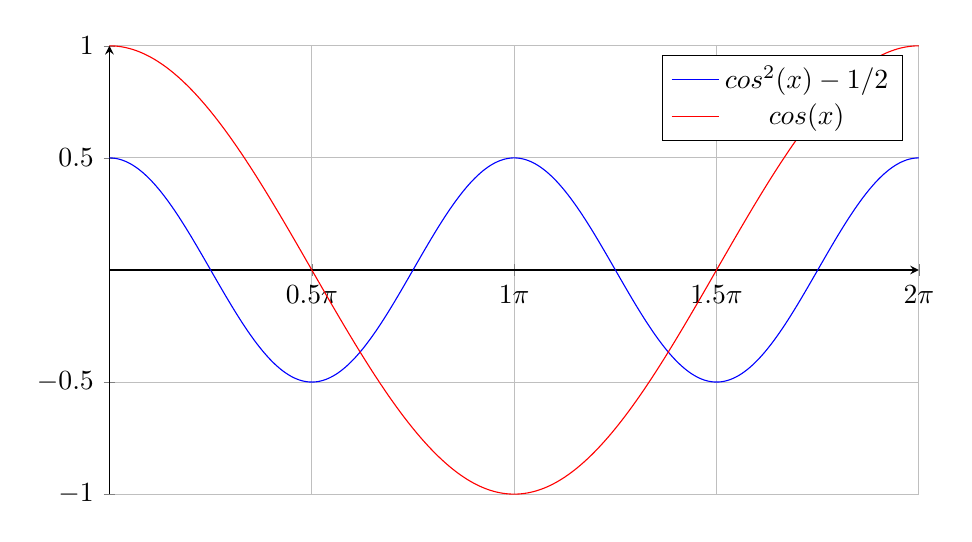
\begin{tikzpicture}
        \begin{axis}
            [
            grid=both,
            axis lines=middle,
            domain=0:2*pi,
            samples=500,
            no marks,
            xticklabels={-2$\pi$,-1.5$\pi$,...$\pi$,2$\pi$},
            xtick={-6.2832,-4.7124,...,6.2832},
            x post scale=1.5
            ]
            \addplot {cos(deg(x))^2 - (1/2)};
            \addlegendentry{$cos^2(x) - 1/2$};
            \addplot {cos(deg(x))};
            \addlegendentry{$cos(x)$};
        \end{axis}
    \end{tikzpicture}
    
    
    So, visually here we can tell that $f(x)$ is less than zero at around $.25\pi \rightarrow 0.75\pi$. Or, in other words from $\frac{\pi}{4}$ to $\frac{3\pi}{4}$. The other period of time that it's less than zero is $\frac{5\pi}{4}$ to $7\frac{\pi}{4}$. This makes sense considering the values we found. It's also important to note that those values at 0 are not included in our interval. So, from this we get the following.
    
    \[\boxed{ \left[ 0, \frac{\pi}{4}\right) \cup \left( \frac{3\pi}{4}, \frac{5\pi}{4}\right) \cup \left( \frac{7\pi}{4}, 2\pi \right]  }\]
\end{solution}


\pagebreak


\begin{problem}[73]
    $cos(2x) \leq 0$
\end{problem}

\begin{solution}
    I'm going to go a little faster on this one. Refer to previous problems if the logic gets hard to follow.
    
    \begin{align}
        \textbf{Part I} && \textbf{Part II} \\
        cos(2x) \leq 0 && 2cos^2(x) - 1 = 0 \\
        2cos^2(x) - 1 \leq 0 && cos(x) = \sqrt{\frac{1}{2}} \\
        \textbf{Let} \; 2cos^2(x) - 1 = f(x) && cos(x) = \pm \frac{\sqrt{2}}{2} \\
        f(x) = 0 && x = \frac{\pi}{4}, \frac{3\pi}{4}, \frac{5\pi}{4}, \frac{7\pi}{4}
    \end{align}
    
    We know our zeroes now, let's make another plot.
    
    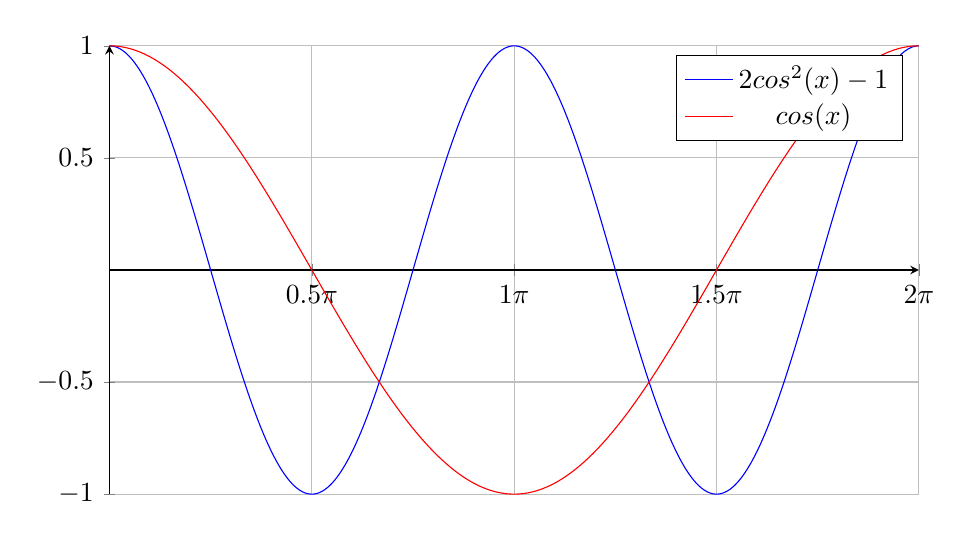
\begin{tikzpicture}
        \begin{axis}
            [
            grid=both,
            axis lines=middle,
            domain=0:2*pi,
            samples=500,
            no marks,
            xticklabels={-2$\pi$,-1.5$\pi$,...$\pi$,2$\pi$},
            xtick={-6.2832,-4.7124,...,6.2832},
            x post scale=1.5
            ]
            \addplot {2 * cos(deg(x))^2 - 1};
            \addlegendentry{$2cos^2(x) - 1$};
            \addplot {cos(deg(x))};
            \addlegendentry{$cos(x)$};
        \end{axis}
    \end{tikzpicture}
    
    Remember that list of values I said were less than zero in problem 72? Funnily enough, our interval will actually be the same as that for this problem! Even by visually inspecting the two plots we can see the areas where they are above and below zero are the same! Therefore we can state our answer. Remember though, our zeroes are included this time! 
    
    \[\boxed{ \left[\frac{\pi}{4}, \frac{3\pi}{4} \right] \cup \left[ \frac{5\pi}{4}, \frac{7\pi}{4} \right]  }\]
\end{solution}
\end{document}